% =================================================================
% FILE: race_methodology_checklist.tex
% PURPOSE: Standalone methodology and checklist for Race Condition Vulnerabilities
% =================================================================

\documentclass[11pt]{article}

% ---------------------------------------------------------------
% PREAMBLE
% ---------------------------------------------------------------
\usepackage[a4paper,margin=2cm]{geometry}
\usepackage{fontspec}
\setmainfont{DejaVu Serif}
\setmonofont{DejaVu Sans Mono}

\usepackage{listings}
\usepackage{xcolor}
\usepackage{enumitem}
\usepackage{titlesec}
\usepackage{hyperref}
\usepackage[breakable,skins]{tcolorbox}
\usepackage{fancyhdr}
\usepackage{amssymb}
\usepackage{tikz}
\usetikzlibrary{arrows.meta,positioning,shapes.geometric,fit,backgrounds}

% Colors
\definecolor{codebg}{RGB}{245,245,245}
\definecolor{httpblue}{RGB}{20,60,110}
\definecolor{causeorange}{RGB}{180,80,0}
\definecolor{checkgreen}{RGB}{0,120,0}
\definecolor{stepblue}{RGB}{0,80,160}
\definecolor{timingcolor}{RGB}{200,50,50}
\definecolor{labblue}{RGB}{20,60,110}

% Listings styles
\lstdefinestyle{code}{
    backgroundcolor=\color{codebg},
    basicstyle=\ttfamily\small,
    frame=single,
    rulecolor=\color{gray},
    columns=fullflexible,
    breaklines=true,
    breakatwhitespace=false,
    showstringspaces=false,
    language=Python,
    keywordstyle=\color{httpblue}\bfseries,
    commentstyle=\color{causeorange}\itshape,
    stringstyle=\color{teal},
    morekeywords={def,queueRequests,handleResponse,RequestEngine,Engine,openGate}
}

\lstdefinestyle{http}{
    backgroundcolor=\color{codebg},
    basicstyle=\ttfamily\small,
    frame=single,
    rulecolor=\color{gray},
    columns=fullflexible,
    breaklines=true,
    breakatwhitespace=false,
    showstringspaces=false,
    language=,
}

\lstset{escapeinside={(*@}{@*)}}

% Headings
\titleformat{\section}{\Large\bfseries\color{httpblue}}{\thesection}{1em}{}
\titleformat{\subsection}{\large\bfseries}{\thesubsection}{1em}{}
\titleformat{\subsubsection}{\normalsize\bfseries\itshape}{\thesubsubsection}{1em}{}

\pagestyle{fancy}
\fancyhf{}
\lhead{Race Condition Vulnerabilities -- Methodology \& Checklist}
\rhead{\thepage}
\setlength{\headheight}{14pt}

% tcolorbox environments
\newtcolorbox{causebox}{
    breakable, colback=orange!5, colframe=causeorange,
    title=Root Cause (Programming Perspective),
    fonttitle=\bfseries, coltitle=white
}

\newtcolorbox{checklistbox}{
    breakable, colback=green!5, colframe=checkgreen,
    title=Checklist,
    fonttitle=\bfseries, coltitle=white
}

\newtcolorbox{stepbox}[1]{
    breakable, colback=blue!4, colframe=stepblue,
    title=Step #1,
    fonttitle=\bfseries, coltitle=white
}

\newtcolorbox{techniquebox}{
    breakable, colback=red!4, colframe=timingcolor,
    title=Timing Technique,
    fonttitle=\bfseries, coltitle=white
}

\newtcolorbox{labbox}[1]{
    breakable, colback=blue!4, colframe=labblue,
    title=#1,
    fonttitle=\bfseries, coltitle=white
}
\hypersetup{colorlinks=true, linkcolor=httpblue, urlcolor=httpblue, citecolor=httpblue}

\setlist[itemize]{leftmargin=*}
\setlist[enumerate]{leftmargin=*}

% Custom commands
\newcommand{\tool}[1]{\textsf{\textbf{#1}}}
\newcommand{\req}[1]{{\color{httpblue}\texttt{#1}}}

% ---------------------------------------------------------------
\title{\textbf{Race Condition Vulnerabilities}\\Methodology \& Checklist}
\author{Eyad Islam El-Taher}
\date{}

\begin{document}
\maketitle
\tableofcontents
\newpage

% =================================================================
\section{Methodology Overview}
% =================================================================

\begin{itemize}
    \item \textbf{Goal:} Identify, confirm, and exploit race condition vulnerabilities across web applications.
    \item \textbf{Approach:} Systematic mapping → collision prediction → probing → timing control → exploitation → confirmation.
    \item \textbf{Key mindset:} Stop thinking in terms of ``one request, one response.'' Every endpoint that touches shared state is really asking: \textit{what happens if this exact code path runs twice, at the same instant, for the same record?}
\end{itemize}

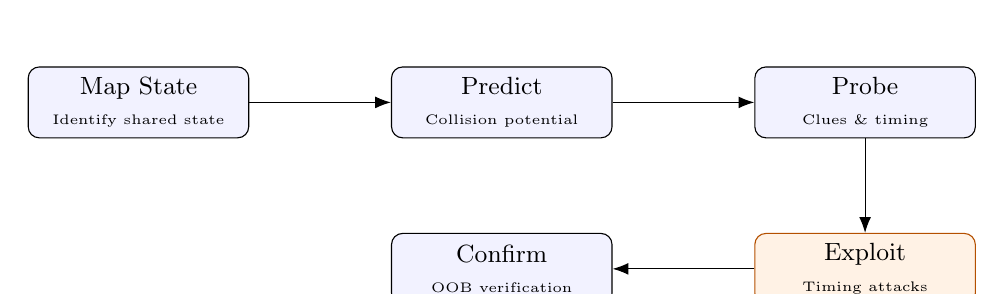
\begin{tikzpicture}[node distance=1.2cm, every node/.style={font=\small, align=center}]
    \node[draw, rounded corners, fill=blue!5, minimum width=2.8cm, minimum height=0.9cm] (map) {Map State\\\tiny{Identify shared state}};
    \node[draw, rounded corners, fill=blue!5, minimum width=2.8cm, minimum height=0.9cm, right=1.8cm of map] (predict) {Predict\\\tiny{Collision potential}};
    \node[draw, rounded corners, fill=blue!5, minimum width=2.8cm, minimum height=0.9cm, right=1.8cm of predict] (probe) {Probe\\\tiny{Clues \& timing}};
    \node[draw, rounded corners, fill=orange!10, draw=causeorange, minimum width=2.8cm, minimum height=0.9cm, below=1.2cm of probe] (exploit) {Exploit\\\tiny{Timing attacks}};
    \node[draw, rounded corners, fill=blue!5, minimum width=2.8cm, minimum height=0.9cm, below=1.2cm of predict] (confirm) {Confirm\\\tiny{OOB verification}};
    
    \draw[-{Latex[length=2mm]}] (map) -- (predict);
    \draw[-{Latex[length=2mm]}] (predict) -- (probe);
    \draw[-{Latex[length=2mm]}] (probe) -- (exploit);
    \draw[-{Latex[length=2mm]}] (exploit) -- (confirm);
\end{tikzpicture}

% =================================================================
\section{Phase 1: Predict Potential Collisions}
% =================================================================

\subsection{Map the Application State}

\begin{checklistbox}
\begin{itemize}
    \item[\checkmark] \textbf{Security-critical endpoints:} Endpoints with no real security/business impact are not worth racing
    \item[\checkmark] \textbf{Collision potential:} Need two or more requests that operate on the \emph{same} underlying record
    \begin{itemize}
        \item Same user session (cookies)
        \item Same resource ID (product, order, account)
        \item Same shared counter (coupon, balance, attempts)
    \end{itemize}
    \item[\checkmark] \textbf{Look for:}
    \begin{itemize}
        \item Coupons/discounts and gift cards
        \item Balances and financial transactions
        \item Login/2FA/OTP attempt counters
        \item Password reset and email-change flows
        \item Invite/registration systems
        \item Any ``one-time'' action
        \item Multi-step checkouts
    \end{itemize}
\end{itemize}
\end{checklistbox}

\subsection{Types of Race Conditions}

\begin{center}
\begin{tabular}{|l|l|l|}
\hline
\textbf{Type} & \textbf{Description} & \textbf{Example} \\
\hline
Limit-Overrun & Check-then-act on a counter & Multiple coupon redemptions \\
Rate-Limit Bypass & Counter check not atomic & Brute-force past lockout \\
Multi-Endpoint & Two different endpoints race & Add-to-cart vs checkout \\
Single-Endpoint & Same endpoint, different values & Email change with two addresses \\
Partial-Construction & Object read mid-creation & Confirm before token stored \\
Time-Sensitive & Predictable token generation & Timestamp-based reset tokens \\
\hline
\end{tabular}
\end{center}

% =================================================================
\section{Phase 2: Probe for Clues}
% =================================================================

\subsection{Initial Probing}

\begin{checklistbox}
\begin{itemize}
    \item[\checkmark] Perform the action normally once, note response and timing
    \item[\checkmark] Repeat the action and compare: does the token/value change each time?
    \item[\checkmark] Is the length constant? (suggests fixed-format hash or ID)
    \item[\checkmark] Send request twice in Repeater sequentially, note response times
    \item[\checkmark] If every response is delayed/serialized under parallel send → suspect \textbf{session-based locking} (PHP native session handler)
    \item[\checkmark] If session locking is masking the race → retest using \textbf{two separate sessions}
\end{itemize}
\end{checklistbox}

\subsection{Token/Parameter Fuzzing}

\begin{checklistbox}
\begin{itemize}
    \item[\checkmark] Try malformed/edge-case values on token-comparison endpoints:
    \begin{itemize}
        \item Missing parameter
        \item Empty string (\texttt{token=})
        \item Empty array (\texttt{token[]=})
        \item Null-equivalent values
    \end{itemize}
    \item[\checkmark] Different error messages reveal how comparison is implemented:
    \begin{itemize}
        \item \texttt{Missing parameter} vs \texttt{Incorrect token} vs \texttt{Forbidden}
        \item \texttt{Array} in error message suggests array was accepted as input
    \end{itemize}
\end{itemize}
\end{checklistbox}

\subsection{Timing Analysis}

\begin{checklistbox}
\begin{itemize}
    \item[\checkmark] Benchmark relative response times between requests you plan to race
    \item[\checkmark] If one is consistently much faster → need deliberate client-side delay
    \item[\checkmark] Fast request must land \emph{inside} slow request's race window
    \item[\checkmark] Use:
    \begin{itemize}
        \item \textbf{Warm connections:} send a throwaway request first
        \item \textbf{Deliberate delay:} add \texttt{sleep()} or use Turbo Intruder's \texttt{gate} control
        \item \textbf{Slow responses:} make remote file respond slowly (for URL-based uploads)
    \end{itemize}
\end{itemize}
\end{checklistbox}

% =================================================================
\section{Phase 3: Timing Techniques}
% =================================================================

\subsection{HTTP/1.1 Last-Byte Synchronization}

\begin{techniquebox}
\begin{itemize}
    \item Send every request in the group \textbf{except the final byte}
    \item Hold each connection open with all requests parked mid-stream
    \item Release the last byte of every request back-to-back
    \item All requests reach application layer within microseconds
\end{itemize}
\end{techniquebox}

\begin{lstlisting}[style=code]
engine.queue(request, gate='race1')
engine.openGate('race1')   # releases withheld final bytes together
\end{lstlisting}

\subsection{HTTP/2 Single-Packet Attack}

\begin{techniquebox}
\begin{itemize}
    \item HTTP/2 multiplexes several requests over one TCP connection
    \item Stuff 20–30 complete requests into a single TCP packet
    \item All arrive at the server in the same instant
    \item Removes network jitter entirely
    \item In Burp: duplicate request 20+ times → \textit{Send group in parallel (single-packet attack)}
\end{itemize}
\end{techniquebox}

\subsection{Bypassing Session-Based Locking}

\begin{techniquebox}
\begin{itemize}
    \item PHP's native session handler processes one request at a time \emph{per session}
    \item This serializes requests, masking race conditions
    \item \textbf{Bypass:} Use two different sessions for two racing requests
    \item Get a fresh session by making a request without a session cookie
    \item Swap the fresh session/CSRF pair into one of the racing requests
\end{itemize}
\end{techniquebox}

% =================================================================
\section{Phase 4: Exploitation}
% =================================================================

\subsection{Pattern 1: Limit-Overrun}

\begin{labbox}\textsc{•}{Pattern: One-time coupon/discount}
\begin{enumerate}
    \item Send \texttt{POST /cart/coupon} with the discount code
    \item Duplicate into a group of 20+ tabs
    \item Send group \textbf{in parallel} (single-packet attack)
    \item Refresh cart — discount applied multiple times
    \item Stack discounts until price under target
\end{enumerate}
\end{labbox}

\begin{lstlisting}[style=code]
# Root Cause Pattern
if not code.used:
    apply_discount(order)
    code.used = True   # Write happens AFTER discount is applied
\end{lstlisting}

\begin{causebox}
If 20 requests reach \texttt{if not code.used} before any reaches the write, all 20 see \texttt{used = False} and all 20 apply the discount. No lock/transaction wraps the check-and-set as one atomic unit.
\end{causebox}

\subsection{Pattern 2: Rate-Limit Bypass}

\begin{labbox}{Pattern: Brute-force past lockout}
\begin{enumerate}
    \item Submit wrong passwords for a user — confirm lockout after 3 attempts
    \item Use Turbo Intruder with single-packet attack
    \item Load password wordlist, set \texttt{username=target}
    \item Fire all guesses in one race window
    \item Watch for 302 redirect (successful login)
\end{enumerate}
\end{labbox}

\begin{lstlisting}[style=code]
# Root Cause Pattern
attempts = get_failed_attempts(username)   # read
if attempts >= 3: return "Locked"
verify_password(username, password)        # slow: DB/hash compare
increment_failed_attempts(username)        # write happens LAST
\end{lstlisting}

\begin{causebox}
Counter stored per-username, increment deferred until after slow password check. N parallel requests = N reads before first write, so effective limit becomes ``N attempts per race window'' instead of 3 total.
\end{causebox}

\subsection{Pattern 3: Multi-Endpoint Race}

\begin{labbox}{Pattern: Add-to-cart vs checkout}
\begin{enumerate}
    \item Identify two endpoints touching same shared state
    \item Build two Repeater groups (add item + checkout)
    \item Send both groups in parallel repeatedly
    \item Check cart/response after each burst
    \item Item added during race window rides into finalized order
\end{enumerate}
\end{labbox}

\begin{lstlisting}[style=code]
# Root Cause Pattern
if cart.total <= user.balance:      # validation step (time T0)
    # --- race window: cart is still mutable here ---
    finalize_order(cart)            # commit step (time T0 + delta)
\end{lstlisting}

\begin{causebox}
Validation and finalization are two separate steps (sometimes separate HTTP requests). Cart can be mutated \emph{after} balance check passed but \emph{before} order confirmed. Any item added during that gap rides into finalized order without being balance-checked.
\end{causebox}

\subsection{Pattern 4: Single-Endpoint Race}

\begin{labbox}{Pattern: Email change with two addresses}
\begin{enumerate}
    \item Duplicate email-change request with different email values
    \item Send both requests \textbf{in parallel} under same session
    \item One request's data may ``win'' the write race
    \item Other request's confirmation token may still be generated
    \item Click confirmation link — address changes to target
\end{enumerate}
\end{labbox}

\begin{lstlisting}[style=code]
# Root Cause Pattern
session['pending_email'] = new_email     # write 1 (request A)
session['pending_email'] = new_email     # write 2 (request B, races A)
send_confirmation(session['pending_email'])   # read — which write "won"?
\end{lstlisting}

\begin{causebox}
Both requests operate on same session-scoped variable with no locking. Final value depends on which write executed last, but confirmation token/email pairing may have captured the other request's data, producing mismatch attacker can exploit.
\end{causebox}

\subsection{Pattern 5: Partial-Construction Race}

\begin{labbox}{Pattern: Confirm account before token stored}
\begin{enumerate}
    \item Study registration flow: user row created, then token stored
    \item Probe \texttt{/confirm} with edge-case values:
    \begin{itemize}
        \item No token → \texttt{Missing parameter}
        \item Empty token → \texttt{Forbidden} (patched)
        \item Empty array \texttt{token[]=} → \texttt{Incorrect token: Array} (accepted!)
    \end{itemize}
    \item Registration is slower than confirmation (benchmark)
    \item Add deliberate delay to confirmation requests
    \item Flood confirmation attempts while registering many users
    \item Watch for \texttt{Account registration successful}
\end{enumerate}
\end{labbox}

\begin{lstlisting}[style=code]
# Root Cause Pattern
user = db.insert_user(username, email, password)   # write 1: row exists, token NULL
token = generate_token()
db.update_user_token(user.id, token)                # write 2: token finally set
\end{lstlisting}

\begin{causebox}
Between write 1 and write 2 the token column is \texttt{NULL}. PHP-style loose comparison can make \emph{array} submitted as \texttt{token[]=} evaluate as equal to uninitialized/\texttt{NULL} stored token. Landing confirmation in that gap confirms account without knowing real token.
\end{causebox}

\subsection{Pattern 6: Time-Sensitive Tokens}

\begin{labbox}{Pattern: Predictable password reset token}
\begin{enumerate}
    \item Trigger password reset — observe token format
    \item Token is same length but different each time
    \item Send two reset requests under different sessions in parallel
    \item If response times match, both emails contain \textbf{same token}
    \item Token is timestamp-based, not cryptographically secure
    \item Use your token, edit \texttt{username} parameter to target
    \item Reset target's password, log in
\end{enumerate}
\end{labbox}

\begin{lstlisting}[style=code]
# Root Cause Pattern
token = md5(username_secret_salt + str(time.time()))
\end{lstlisting}

\begin{causebox}
Token generation relies on high-resolution timestamp instead of CSPRNG. If two reset requests processed at same server timestamp (achieved by racing under separate sessions to dodge PHP's per-session request lock), they hash to identical token regardless of which username triggered them.
\end{causebox}

% =================================================================
\section{Phase 5: Impact Confirmation}
% =================================================================

\begin{checklistbox}
\begin{itemize}
    \item[\checkmark] \textbf{Coupon abuse:} Refresh cart, verify discount applied multiple times
    \item[\checkmark] \textbf{Rate-limit bypass:} Check for 302 redirect (successful login)
    \item[\checkmark] \textbf{Multi-endpoint:} Check cart state, order confirmation, balance
    \item[\checkmark] \textbf{Single-endpoint:} Verify email changed, token worked
    \item[\checkmark] \textbf{Partial construction:} Log in with registered account
    \item[\checkmark] \textbf{Time-sensitive:} Reset target password, log in
    \item[\checkmark] \textbf{Out-of-band:} Check inbox, refresh cart, recheck balance
    \item[\checkmark] \textbf{Don't trust status codes alone} — a collision doesn't always produce an obviously different response
\end{itemize}
\end{checklistbox}

% =================================================================
\section{Complete Testing Checklist}
% =================================================================

\begin{checklistbox}
\subsection*{Phase 1: Predict Potential Collisions}
\begin{itemize}
    \item[$\square$] Map all endpoints that touch shared state (sessions, database rows, counters)
    \item[$\square$] Identify security-critical endpoints (coupons, balances, login, password reset)
    \item[$\square$] Look for collision potential: same session, same resource, same counter
    \item[$\square$] Note any ``one-time'' actions or multi-step workflows
\end{itemize}

\subsection*{Phase 2: Probe for Clues}
\begin{itemize}
    \item[$\square$] Perform action normally once, note response and timing
    \item[$\square$] Repeat and compare token/value changes
    \item[$\square$] Send two requests sequentially in Repeater, note response times
    \item[$\square$] Test with malformed/edge-case parameter values
    \item[$\square$] Check for session-based locking masking the race
\end{itemize}

\subsection*{Phase 3: Choose Timing Technique}
\begin{itemize}
    \item[$\square$] HTTP/2 available? → Single-packet attack
    \item[$\square$] HTTP/1.1 only? → Last-byte synchronization
    \item[$\square$] Session locking masking? → Use two separate sessions
    \item[$\square$] Need controlled delay? → Turbo Intruder with \texttt{gate} control
\end{itemize}

\subsection*{Phase 4: Exploitation}
\begin{itemize}
    \item[$\square$] \textbf{Limit-Overrun:} Send same endpoint repeated in parallel
    \item[$\square$] \textbf{Rate-Limit Bypass:} Fire guesses in one race window
    \item[$\square$] \textbf{Multi-Endpoint:} Race two different endpoints touching same record
    \item[$\square$] \textbf{Single-Endpoint:} Race same endpoint with different parameter values
    \item[$\square$] \textbf{Partial-Construction:} Flood confirm requests during registration
    \item[$\square$] \textbf{Time-Sensitive:} Race requests to generate matching tokens
\end{itemize}

\subsection*{Phase 5: Confirmation}
\begin{itemize}
    \item[$\square$] Verify out-of-band (inbox, cart state, balance, admin panel)
    \item[$\square$] Don't trust status codes alone
    \item[$\square$] Retry with reordered request sequencing
    \item[$\square$] Warm connection with throwaway request first
    \item[$\square$] Document exact payload and conditions
\end{itemize}
\end{checklistbox}

% =================================================================
\section{Turbo Intruder Templates}
% =================================================================

\subsection{Template 1: Single Request Repeated}

\begin{lstlisting}[style=code]
def queueRequests(target, wordlists):
    engine = RequestEngine(endpoint=target.endpoint,
                            concurrentConnections=30,
                            requestsPerConnection=30,
                            pipeline=False)
    for i in range(30):
        engine.queue(target.req, i)
        engine.queue(target.req, target.baseInput, gate='race1')
    engine.start(timeout=5)
    engine.openGate('race1')
    engine.complete(timeout=60)

def handleResponse(req, interesting):
    table.add(req)
\end{lstlisting}

\subsection{Template 2: Two Different Requests Racing}

\begin{lstlisting}[style=code]
def queueRequests(target, wordlists):
    engine = RequestEngine(endpoint=target.endpoint,
                            concurrentConnections=30,
                            requestsPerConnection=100,
                            pipeline=False)
    request1 = '''
POST /target-URI-1 HTTP/1.1
Host: <TARGET>
Cookie: session=<SESSION>

parameter=value
    '''
    request2 = '''
GET /target-URI-2 HTTP/1.1
Host: <TARGET>
Cookie: session=<SESSION>
    '''
    engine.queue(request1, gate='race1')
    for i in range(30):
        engine.queue(request2, gate='race1')
    engine.openGate('race1')
    engine.complete(timeout=60)

def handleResponse(req, interesting):
    table.add(req)
\end{lstlisting}

\subsection{Template 3: Single-Packet Attack (HTTP/2)}

\begin{lstlisting}[style=code]
def queueRequests(target, wordlists):
    engine = RequestEngine(endpoint=target.endpoint,
                            concurrentConnections=1,
                            engine=Engine.BURP2)   # single-packet attack
    for word in open('/path/to/wordlist.txt'):
        engine.queue(target.req, word.rstrip(), gate='race1')
    engine.openGate('race1')

def handleResponse(req, interesting):
    table.add(req)
\end{lstlisting}

% =================================================================
\section{Tools Reference}
% =================================================================

\begin{center}
\begin{tabular}{|l|l|}
\hline
\textbf{Tool} & \textbf{Purpose} \\
\hline
Burp Suite Repeater (2023.9+) & Send group in parallel (single-packet attack) \\
Turbo Intruder & Fine-tuned timing control, scriptable \\
Burp Collaborator & Out-of-band verification \\
Burp Inspector & Decode/analyze tokens \\
PayloadsAllTheThings & Reference payloads \\
\hline
\end{tabular}
\end{center}

% =================================================================
\section{Common Pitfalls \& How to Avoid Them}
% =================================================================

\begin{itemize}
    \item \textbf{Pitfall:} Testing only one endpoint, missing multi-endpoint races
    \begin{itemize}
        \item \textbf{Solution:} Map all endpoints touching the same shared state
    \end{itemize}
    
    \item \textbf{Pitfall:} Assuming session locking means no race is possible
    \begin{itemize}
        \item \textbf{Solution:} Retest with two separate sessions
    \end{itemize}
    
    \item \textbf{Pitfall:} Not checking for partial-construction sub-states
    \begin{itemize}
        \item \textbf{Solution:} Fuzz token-comparison endpoints with edge-case values
    \end{itemize}
    
    \item \textbf{Pitfall:} Only testing same-session races
    \begin{itemize}
        \item \textbf{Solution:} Test cross-session races where different users share a resource
    \end{itemize}
    
    \item \textbf{Pitfall:} Trusting status codes alone for confirmation
    \begin{itemize}
        \item \textbf{Solution:} Verify out-of-band (inbox, cart, balance)
    \end{itemize}
    
    \item \textbf{Pitfall:} Giving up after one failed burst
    \begin{itemize}
        \item \textbf{Solution:} Retry with reordered sequencing, connection warming, delays
    \end{itemize}
    
    \item \textbf{Pitfall:} Not benchmarking relative response times
    \begin{itemize}
        \item \textbf{Solution:} Add deliberate delay to faster requests
    \end{itemize}
\end{itemize}

% =================================================================
\section{Prevention Recommendations}
% =================================================================

\begin{itemize}
    \item \textbf{Atomic check-and-act:} Wrap read, decision, and write in single DB transaction
    \item \textbf{Row-level locking:} Use \texttt{SELECT ... FOR UPDATE} around critical sections
    \item \textbf{Idempotency keys:} Unique constraints so second insert fails
    \item \textbf{Avoid session-level ambiguity:} Don't share one mutable variable across operations
    \item \textbf{CSPRNG tokens:} Never use timestamps for security tokens
    \item \textbf{Rate-limit at infrastructure layer:} WAF/gateway-level limiter
    \item \textbf{Avoid mutable sub-states:} Validate and finalize in one atomic operation
\end{itemize}

% =================================================================
\section{References}
% =================================================================

\begin{itemize}
    \item PortSwigger Web Security Academy: \url{https://portswigger.net/web-security/race-conditions}
    \item PortSwigger Research — \textit{Smashing the State Machine: The True Potential of Web Race Conditions}, James Kettle, Black Hat USA 2023
    \item PayloadsAllTheThings — Race Condition: \url{https://github.com/swisskyrepo/PayloadsAllTheThings}
    \item Turbo Intruder: \url{https://github.com/PortSwigger/turbo-intruder}
    \item Josip Franjkovic — \textit{Race conditions on the web} (2016)
    \item Laxman Muthiyah — \textit{Instagram Password Reset Mechanism Race Condition}
\end{itemize}

\end{document}